\chapter{Background}
% 2000 words
	The project involved analysis of brain connectivity graphs computed from \ac{MEG} recordings. The following chapter depicts background knowledge needed for a better understanding of chosen methodologies.

	% AD - complete
	\section{Alzheimer's Disease}
	Increasing evidence points that the accumulation of beta-amyloid (A\(\beta\)) plaques in brain tissue is the most likely cause of \ac{AD} \autocite{Cummings2004}. Neuronal death is believed to be an effect of this increase in plaques. The only precise way of diagnosing \ac{AD} is by post-mortem examination of cortical tissue, but this is useful only in disease confirmation after death \autocite{Khachaturian1985}. Treatment in earlier phases of the disease can prove beneficial in delaying disorder symptoms. There are four main stages of \ac{AD}: \ac{MCI}, Mild and Moderate \ac{AD} and Severe \ac{AD}. In the \ac{MCI} stage, the patient experiences memory loss as a main symptom \autocite{Morris2001}. An area of disease diagnostic that shows promising results is represented by neuroimaging biomarkers \autocite{Weiner2013,Filippi2011,Sperling2011}. 


	% MEG 
	\section{The Physics of \ac{MEG}}
		\ac{MEG} is a noninvasive neuroimaging technique that measures perturbations occurring in the magnetic field produced by populations of neurons in the brain \autocite{LopesdaSilva2013}. Figure~\ref{fig:MEGsignal} shows that magnetic fields are generated by neuronal currents and picked up by the \ac{MEG} sensors. The main advantage of this technology is the high temporal resolution (1-100 Hz). Compared to \ac{EEG} that records electrical impulses at the scalp level, \ac{MEG} is more precise as magnetic signals suffer less distortion by the scalp and skull \autocite{LopesdaSilva2013}. 

		% ?? REFERENCE IF PERMISSION GRANTED
		\begin{figure}
		    \centering
		    \includegraphics[width=0.8\textwidth]{magneticfield-origin}
		    \caption{Magnetic fields are generated by the electrical activity of neurons (adapted from \textcite{Washington}).}
		    \label{fig:MEGsignal}
		\end{figure}

		% brief history of MEG
		% Explain Physics of MEG (vid); 2 physical phenomena are at the core of MEG technology; one is superconductivity and the other is quantum interference. explain them.
		The main technological achievement that lies at the foundation of \ac{MEG} technology is the \ac{SQUID} \autocite{Vrba2001}. This is a very sensitive magnetic detector based on two physical phenomena: superconductivity and quantum tunnelling. It was first used by \textcite{Cohen1972} in the context of a single-channel recording. Today's \ac{MEG} systems can have several hundreds of channels, where each channel corresponds to its own \ac{SQUID} \autocite{Vrba2001}.

		% MEG noise sources
		There are also several disadvantages of \ac{MEG} that one should be aware of. In contrast to having high temporal resolution, \ac{MEG} also has low spatial resolution (order of millimetres or centimetres) \autocite{LopesdaSilva2013}. One of the most pervasive problems in \ac{MEG} recordings is additive noise. Sources of noise can come from the exterior of the sensor helmet such as cardiac artefacts \autocite{Jousmaki1996} and power lines \autocite{Keshtkaran2014} or from the interior such as ocular artefacts caused by blinks \autocite{Jousmaki1996}. These should be minimised in the preprocessing stage of any analysis. The final problem mentioned here is the volume conduction problem that appears when activity from the same source is registered by multiple \ac{MEG} sensors because of their proximity \autocite{LopesdaSilva2013}.

		
	\section{Resting-State Synchronisation}
	% theory - Default Mode Network paper (no graphs)
	Traditionally, \ac{MEG} signals can be grouped in a number of frequency bands: infraslow (<0.2 Hz), \(\delta\) (0.2-3.5 Hz), \(\theta\) (4-7.5 Hz), \(\alpha\) and \(\mu\) (8-13 Hz), \(\beta\) (14-30 Hz), \(\gamma\) (30-90 Hz) and high-frequency oscillations (>90 Hz) \autocite{LopesdaSilva2013}. When populations of neurons share the same firing patterns, neural oscillations arise. Cognitive functions such as memory are believed to rely on these synchronisation patterns between different regions of the brain \autocite{Schnitzler2005, Gusnard2001}. The \ac{DMN} is a network of brain regions that is believed to be active during resting states, when the person is not actively engaged with a certain task \autocite{Raichle2001}. Since the introduction of this hypothesis, resting-state studies have been successful in identifying correlations in the same brain regions across subjects \autocite{Damoiseaux2006,Beckmann2005,Andrews-Hanna2010}.

	As \ac{AD} affects memory, the next step was to try to find differences between the healthy population and patients. Several studies have found significant differences between these groups, where connectivity in \ac{AD} patients was lower than in control subjects \autocite{Stam2006,Greicius2004,Sheline2010}. The next section introduces graph theory as a relatively new paradigm for brain network analysis \autocite{Stam2012}.

	\section{Connectivity Graphs}
	% network analysis is a new way to compare the disruptions
	Quantitative analysis of brain networks can be obtained using graph theory \autocite{sporns2011networks}. Mapping states of biological networks to corresponding graph measures would be instrumental in disease diagnosis and development.

	A graph is a structure composed of a set of nodes or vertices and a set of edges. The nodes are connected by the edges. When referring to brain graphs, nodes are mapped to anatomical regions and edges specify a connectivity function. This function can be either structural or functional. The structural function describes the anatomical connections of the nervous system and employs \ac{DTI} and tractography \autocite{Jones2011}. \ac{FC} depicts neurophysiological patterns and is explored using \ac{MEG}, \ac{EEG} or \ac{MEG} technologies. Figure~\ref{fig:structfunctnetworks} shows a high-level scheme of extracting graphs from brain signals. Particular attention should be given to \textit{Step 2}, where the association between nodes is computed. In \ac{FC}, the synchronisation measure just describes statistical correlations between different brain regions and makes no statement about underlying causal effects \autocite{sporns2011networks}. 

	\begin{figure}
		    \centering
		    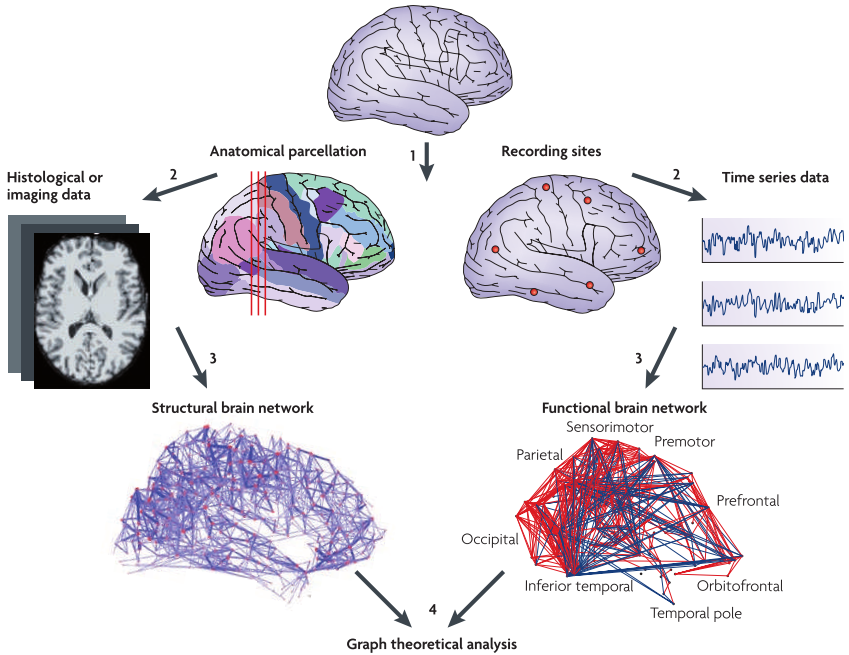
\includegraphics[width=0.95\textwidth]{structfunctnetworks}
		    \caption{Structural and functional brain networks (from \textcite{Bullmore2009}). Step 1 implies identification of graph nodes. This consists of anatomical regions in case of \ac{DTI} and electrodes in case of \ac{EEG} or \ac{MEG}. Step 2 computes a correlation measure between nodes. Step 3 creates an association matrix which holds the correlation strengths between pairs of vertices. Graph measures are computed in the final step.}
		    \label{fig:structfunctnetworks}
	\end{figure}   

	\section{Graph Theory}
	This sections aims to introduce a number of graph features relevant to the current study. A comprehensive review of more complex measures can be found in \autocite{Rubinov2010}.

	Node degree is one of the simplest graph measures. This is given by the number of edges that link a node to the rest of the graph. Another basic graph measure is node centrality. This refers to the number of shortest paths between the other pair of nodes in the network that pass through a specific node. High-centrality measures are critical for fast communication. Network hubs are vertices with either high centrality or high degree. Figure~\ref{fig:graphmeasures} provides an overview of some of the measures.  
	
	The clustering coefficient quantifies local segregation. It refers to how densely connected is a node relative to its neighbours. A high value for this measure indicates that a cluster has been found. The average shortest path length, also called the \ac{L}, is calculated by taking the average number of edges in the shortest paths between every node pair in the graph. This measure can also be found under the name of unnormalised path length. The normalised path length is obtained by dividing \ac{L} by the average path length of a random graph. Random graphs are introduced in the next subsection. 

	A graph is said to have high modularity if it is formed of subgraphs (modules) that display high intraconnectivity and low interconnectivity (connection between subgraphs). 

	\begin{figure}
		    \centering
		    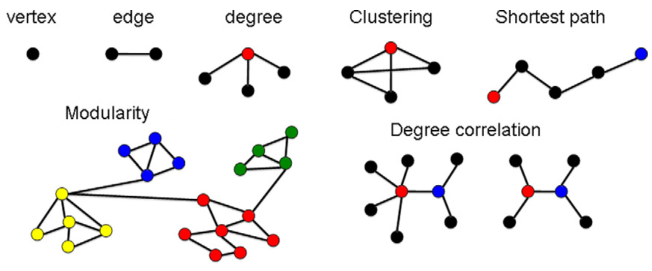
\includegraphics[width=0.8\textwidth]{graphmeasures}
		    \caption{Graph measures (adapted from \textcite{Stam2012}). The red node in the \textit{degree} graph has a degree of three. For the \textit{shortest path graph}, a minimum of four edges need to be traversed from the red node to the blue node which yields a shortest path of four. Four modules can be seen in the \textit{modularity} graph.}
		    \label{fig:graphmeasures}
	\end{figure}   

	\textcite{Watts1998} introduced the idea of "small-world" networks which maintain an equilibrium of high clustering and short paths. Brain networks have been hypothesised to posses this property as a consequence of needing to balance infrastructure costs (building neural paths and maintaining them) and high connectivity between brain regions. Fast local computation and integration of information is achieved using the \ac{SW} topology \autocite{Bullmore2009}. Figure~\ref{fig:smallworld} compares the \ac{SW} network with two other networks.

	\begin{figure}
		    \centering
		    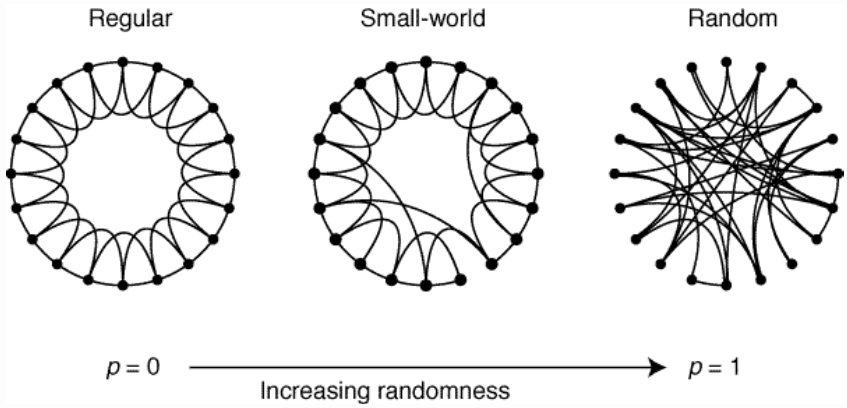
\includegraphics[width=0.8\textwidth]{smallworld}
		    \caption{Basic network types (from \textcite{Watts1998}). Each node of a network is initially connected to its four neighbours. The network is highly clustered and the majority of path lengths between nodes are high. With a probability \textit{p}, edges are disconnected and reattached to a random node. For \textit{p}=1, all of the edges will be reconnected which would result in a random network. This network type lost the high clustering property. For value of \textit{p} between 0 and 1, the network maintains the high clustering quality and depicts small path lengths.}
		    \label{fig:smallworld}
	\end{figure}   

	
	\section{Network Measures as Biomarkers in AD}
	% AD studies (from section 1.2: Graph analysis of AD brain...)
	Analysis of \ac{AD} brain networks using graph theory is a relatively recent research endeavour. Two reviews that describe studies that focused exclusively on \ac{AD} are the ones by \textcite{He2009} and \textcite{Xie2011}. Findings of 13 studies that explored graph metrics in \ac{AD} were listed in the review by \textcite{Tijms2013}. They found that connectivity decreases in \ac{AD} graphs. Common graph characteristics were identified by most of the studies, but there are cases where properties are inconsistent across results.

	Previous studies reported a decline in clustering coefficients in \ac{AD} graphs \autocite{He2009,DeHaan2012a}. The research by \textcite{Stam2004} was one of the first to show that brain networks in healthy subjects have the \ac{SW} property. All studies reviewed in \textcite{Tijms2013} reported that \ac{AD} networks possess the \ac{SW} property and 3 out of 13 studies described a decline in the \ac{SW} value in \ac{AD} networks, with a possible explanation of path length increase. The reported normalised path lengths in \textcite{Tijms2013} were inconsistent. The connection between path length and \ac{SW} property in \ac{MCI} and \ac{AD} patients was superficially investigated in the past \autocite{Tijms2013}. 
	Modularity in \ac{AD} was explored in only a single study which found a fewer number of modules in \ac{AD} networks \autocite{DeHaan2012b}. In the same study, modularity in the \(\theta\) band was increased.    

	Result incompatibilities between studies may be caused by lack of standardised techniques for creating \ac{FC} graphs \autocite{Tijms2013}. Another possible limitation is the small sample sizes employed in the studies. For research that aims to compare three groups such as the one in this project (i.e.\ \ac{AD}, \ac{MCI} and \ac{CS}), larger sample sizes are needed.  

	% we look at global measures -> global approach to characterise networks

	\begin{figure}
		    \centering
		    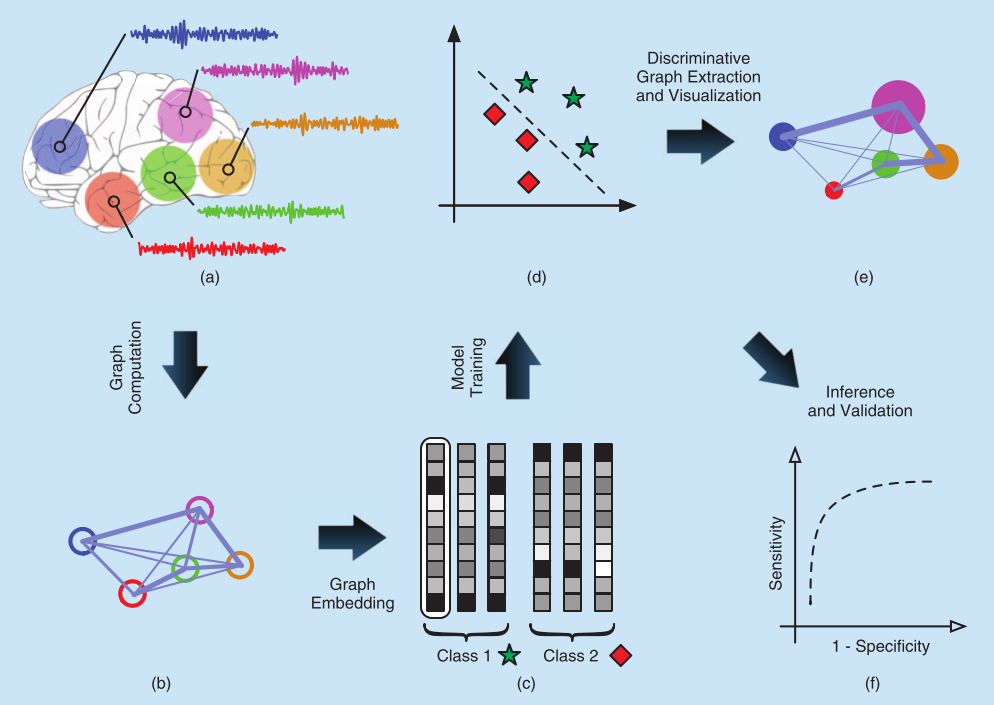
\includegraphics[width=0.9\textwidth]{MLbraingraphs}
		    \caption{Scheme for predictive analysis using brain graphs (from \textcite{Richiardi2013}). In a), imaging data is arranged in regions of interest with each region having corresponding time series. b) A graph is computed from the signals in which vertices correspond to brain regions and edges represent correlations between these regions. c) The graphs are organised in vector structures. d) The vectors are used as input for machine learning algorithms. e) Visualisation of interesting patterns is performed so results can be better interpreted. f) Model evaluation is done in the last stage to assess algorithm quality.}
		    \label{fig:MLbraingraphs}
	\end{figure}

	In addition to studies that looked only at comparing network measures in \ac{AD}, another category distinguishes itself by trying to use machine learning techniques on computed graph features and subsequently performing classification of individuals \autocite{Jie2014,Chen2011,Zhou2011}. The goal is to bring this research into clinical settings for illness diagnosis purposes. A pipeline schema of a project employing graph analysis in a machine learning setting can be seen in Fig.~\ref{fig:MLbraingraphs}. 

	% bit of background about past papers using ML for classification
	% utility of graphical metrics as diagnostic markers

	This project brought together graph analysis of \ac{FC} networks and classification techniques with the aim of furthering research into network-based diagnosis procedures in \ac{AD}.
	% then: in this project we applied graph analyis to compare \ac{FC} networks between AD, MCI and controls. we examined 

\section*{Conclusion}
	This chapter started by describing \ac{AD} and why research in this area is important. Afterwards, an overview of \ac{MEG} was provided as this is the imaging technique used to acquire the data for this project. Lastly, an overview of the state-of-the-art research in graph analysis applied to \ac{AD} was presented. The next chapter describes the specific techniques used to tackle the problem of finding dissimilarities between \ac{AD} patients and healthy people.